% !TeX TS-program = lualatex
% !TeX encoding = UTF-8
% !TeX spellcheck = de_DE
\documentclass[fontsize=12pt,paper=a4,ngerman]{scrarticle}
\author{Justus Gottfried Hache} % Bitte Autor anpassen. Er wird auch in die PDF Metadaten übernommen
\usepackage{sse}
\usepackage{subcaption}

\begin{document}

\makeatletter
\begin{titlepage}
    
\includegraphics[scale=0.6]{pics/logo/TUD-blue.pdf}
    \vspace*{\fill}

	\centering
    % Falls ihr einen grafischen Algorithmus oder sonstige Darstellung habt, fügt doch gern ein Bild ein
    \includegraphics[width=0.4\textheight]{example-image-a} 
	
	\vspace{2em}
	{\LARGE\bfseries Schaltkreis"~ und Systementwurf\par}
    \vspace{1em}
    {\large\bfseries Praktikumsbericht\par}
	\vspace{4em}
	{\large \@author\ (Matrikelnummer)\par\vspace{2em}}
    {\scshape\large Studiengang Informationssystemtechnik \par}
    {\scshape\large Fakultät Elektrotechnik und Informationstechnik \par}
    {\scshape\large Technische Universität Dresden \par}
	\vfill
	{\today\par} % Bottom of the page
\end{titlepage}
\makeatother % titlepage ist eine seperate Datei

% Die Rückseite des Deckblatts sollte immer leer sein
\begingroup
\pagestyle{empty}
\null
\newpage
\endgroup

\tableofcontents % Inhaltsverzeichnis einfügen
\clearpage

% Hier kommt der Inhalt
\section{Einleitung}
Diese Arbeit dokumentiert das Design eines double-percision FFT-ASICs er wurde
für das Modul „Schaltkreis und Systementwurf“ entwickelt. Die Aufgabenstellung
umfasst dabei die Analyse des gewählten Algorithmus, eine sequentielle
Referenzimplementierung, planung der Implementierung in Hardware mithilfe von
Registertransferfolgen, sowie die tatsächliche Implementierung mit dem Cadence
Design Framework 2. Im finalen schritt wird das Design syntetisiert, simuliert
und verifiziert.

Die Fourier Transformation ist eine der wichtigsten Funktionen in der heutigen
Zeit. Sie wird für Komprimierungsalgorithmen, Audio und Bildbearbeitung,
Analyse von Signalen, Übertragung von Signalen und noch vielen anderen
Bereichen verwendet. Die zentrale Eigenschaft der Fourier Transformation ist
dabei, aus einer zeitlichen Folge die Amplituden der Frequenzkomponenten zu
berechnen. Lange Zeit war es nur möglich, die diskrete Version der Fourier
Transformation mit einer Laufzeit von $O = N^2$ zu berechnen. Erst in den 60er
Jahren änderte sich dies mit einem der Schnellen Fourier Transformation,
beschrieben in Die Zentrale Erkenntnis dabei war, dass man sich durch die
periodische Natur der Exponentialfunktion viele Rechnungen sparen konnte. In
ihrer Arbeit beschreiben Colley und Turkey, wie durch umformen der gleichungen
die Fourier Transformation so geschrieben werden kann, dass nun eine Laufzeit
von $O=N\log_N$erreicht werden kann. Dies ermöglicht es auch lange Folgen mit
hoher Frequenzauflösung zu berechnen und heutzutage z.B. die Verwendung in
Komprimierungsalgorithmen und die Fähigkeit in Echtzeit auf eingebetteten
systemen zu laufen.Diese Arbeit wird sich damit befassen, wie man einen AISC
(Application Specific Integrated Circuit) erstellen kann, welcher diese
Berechnung noch schneller durchführen kann, als es ein Prozessor in gleicher
Technologie könnte.

Zitiert wird so: \autocite{munafo_escape_2023}. Die \texttt{.bib} Datei wurde
mit \href{https://www.zotero.org/}{Zotero} erzeugt. Bitte beim Export auf das
neue Format bib\textbf{la}tex achten.

\section{Beschreibung des Algorithmus}
Wie in der Einleitung beschrieben, berechnet die FFT effizient aus einer
Zeitlichen Folge an Werten die Frequenzkomponenten. Die finale Implementierung
ist außerdem darauf ausgelegt, dass die Berechnung in-place stattfindet, also
kein Zusätzlicher Speicher als der Eingabespeicher, welcher gleichzeitig
Ausgabespeicher ist, benötigt wird.

\paragraph{Eingabe}
Der Algorithmus benötigt als Eingabe eine Liste an Werten, welche in
gleichmäßigen Abständen aufgenommen wurden und als weitere Eingabe muss die
länge der Liste angegeben werden. Die Länge der Liste kann dabei nur eine
Potenz von 2 sein. Sollte die Länge der Zahlenfolge kürzer sein, so muss der
restliche Speicher mit Nullen aufgefüllt werden.
%TODO: wie verhält es sich mit den Adress umdrehen?

\paragraph{Ausgabe}
Der Algorithmus liefert eine Liste an Werten, welche den Amplituden der
Frequenzanteile entspricht. Diese Liste hat dabei die gleiche Länge, wie die
Eingabe.
\paragraph{Implementierung}
Ein einfacher weg, die FFT zu veranschaulichen ist der rekursive ansatz. Dieser
funktioniert, indem die Originale Zahlenfolge in 2 Teile zerlegt wird, ein Teil
mit den Graden Indizes und ein Teil mit den ungeraden. Für jeden dieser Teile
wird nun selbst eine FFT berechnet, die Ergebnisse werden schließlich
miteinander verrechnet. Wenn die beiden vorherigen Ergebnisse $E[k]$ und $O[k]$
sind, gilt dann für das Gesamtergebnis $X$ mit der Länge $N$:
\begin{equation}
	\begin{split}
		X[k] = E[k] + W^k_N O[k]     \\
		X[k+N/2] = E[k] - W^k_N O[k] \\ k = 0, \ldots , N/2-1
	\end{split}
\end{equation}

Man benötigt also für die Kombination $N$ komplexe Multiplikationen und
Additionen. Durch wiederholtes Teilen zerlegt man die Zahlenfolge nun solange
bis nur noch ein Element übrig ist. Dies wird erreicht, nach $\log_2N$ Teilen.
Interessanterweise ist die Teilung in 2 Teile nicht der Effizienteste Weg, wenn
man nur auf die Komplexen Multiplikationen schaut. Laut dem originalem Paper
TODO: reference ist eine Teilung in 3 Teile $6\%$ effizienter, eine Teilung in
4 gleich schnell im Vergleich zu einer Teilung in 2. Allerdings Bringt die
Teilung in 2 deutlich vereinfachungen der Speicherung und Adressberechnung auf
binärkomputern, sodass heutzutage meist eine Teilung in 2, einige praktische
Implementierungen TODO:reference aber auch eine Teilung in 4 für eine bessere
Hardwarenutzung verwenden. Die Referenzimplementierung TODO: link verwendet
eine sequentielle Version dieses Algorithmus. Dabei wird jedes Mal Teilen einer
neuen „Stufe“ zugeordnet. Die erste Stufe kombiniert dann $N$ Teile, zu $N/2$
die letzte Stufe kombiniert lediglich $2$. Dadurch kann eine feste Schleife
erstellt werden, welche den Anfangsindex, der jeweiligen in einer Stufe
berechnet und in einer zweiten schleife, wird dann durch die Elemente eines
Teils gegangen.
\subsection{Arithmetik}
Was zum Rundungsverhalten/Abweichungen erklären, usw.

\section{Entwurf}
\subsection{Ablaufdiagramm}
In Diagramm \ref{fig:flowchart} ist der Programmablauf graphisch dargestellt.
Für eine performante Implementierung in Hardware gestaltet sich vor allem die 3
ineinanderliegenden Schleifen, welche in der Finalen implementierung teilweise
parallel ausgeführt werden müssen. Im Ablaufdiagramm wurden folgende Variablen
verwendet:

\begin{itemize}
	\item $len$ = der Logarithmus zur Basis 2 der konfigurierbaren Länge der Datenserie,
	\item $N$ = die Länge der Datenserie am Eingang,
	\item $stagepow$ = 2 hoch die aktuelle Stufe. Wird als counter für den äußeren loop verwendet.
	\item $half$ = Hälfte von $stagepow$, oder der Wert aus der vorherigen Schleifeniteration.
	\item $k$ = Zähler der mittleren Schleife.
	\item $j$ = Zähler der inneren Schleife.
	\item $omega$ = Komplexe Zahl, entspricht $W^k_N$ aus Kapitel Implementierung
	\item $domega$ = Komplexe Zahl, entspricht $W^1_N$ aus Kapitel Implementierung.
	\item $t$,$u$ = Komplexe Hilfsvariablen
\end{itemize}
\begin{figure}[h]
	\label{fig:flowchart}%TODO: this ref is not working right now
	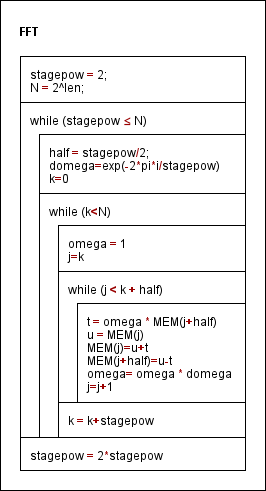
\includegraphics{pics/FFT_flowchart.png}
	\centering
\end{figure}
\subsection{Unoptimierter Datenflussgraph}
In Diagramm \ref{fig:unoptimized_datapath} is eine erste Datenpfadarchitektur
dargestellt, welche als Startpunkt des Entwurfes dient. Prinzipiell kann man
mit dieser Architektur alle Operationen ausführen, die für die Schnelle
Fouriertransformation nötig wären. Eine solche Ausführung wäre allerdings nicht
sonderlich schneller, als eine Implementierung auf einem üblichen Prozessor.

\begin{figure}[ht]
	\centering
	\label{fig:unoptimized_datapath}%TODO: this ref is not working right now
	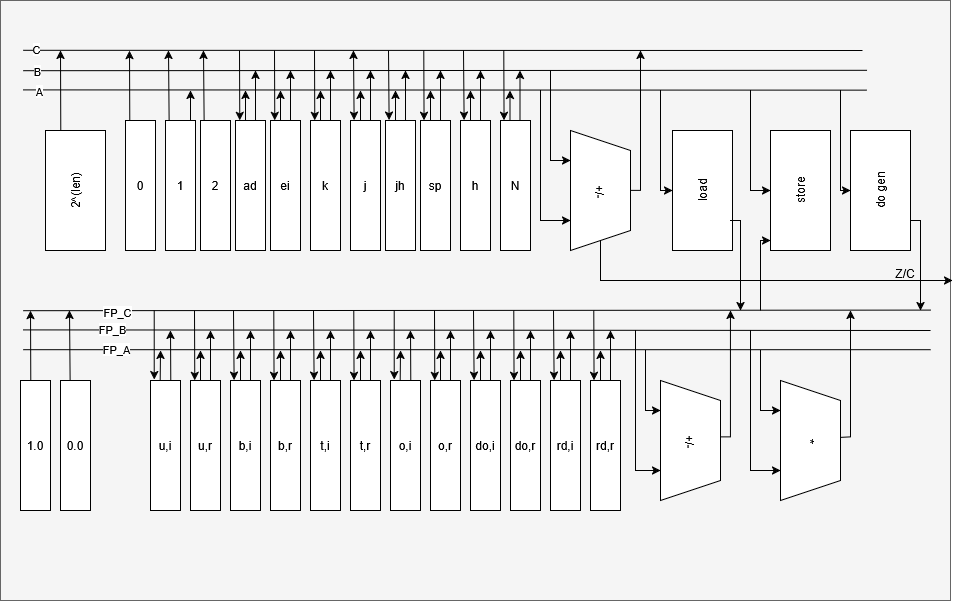
\includegraphics[width=0.8\textwidth]{pics/Datapath architecture.drawio.png}
\end{figure}
\subsection{Unoptimierte FSM}
Um die in Diagramm \ref{fig:unoptimized_datapath} dargestellte
Datenpfadarchitektur zum berechnen einer Fourier zu verwenden, müssen die
verschiedenen möglichen Datentransfers mit einem Endlichen Zustandsautomat
(engl. Finite State Machine, FSM) gesteuert werden. Dieser wird im Folgenden
mithilfe von Registertransferfolgen ersetllt. Dieser unoptimierte
Zustandsautomat ist jedoch sehr groß, sodass wir die Funktionen komplexe
Multiplikation, Addition sowie Subtraktion abgetrennt betrachten.

In der Registertransferfolge \ref{fig:complex_operations_RFD} sind jeweils die
Zustände, welche für Komplexe Addition, Subtraktion und Multiplikation
notwendig sind dargestellt. Die Parameter a,b und c stehen dafür für zwei
Eingangs- und ein Ausgangsregisterpaar mit je einem FP64 Register für komplexen
und reellen Teil. Schon hier wird deutlich, wie viele Takte eine einzelne
komplexe Multiplikation einnehmen kann.

\begin{figure}
	\centering
	\label{fig:complex_operations_RFD}
	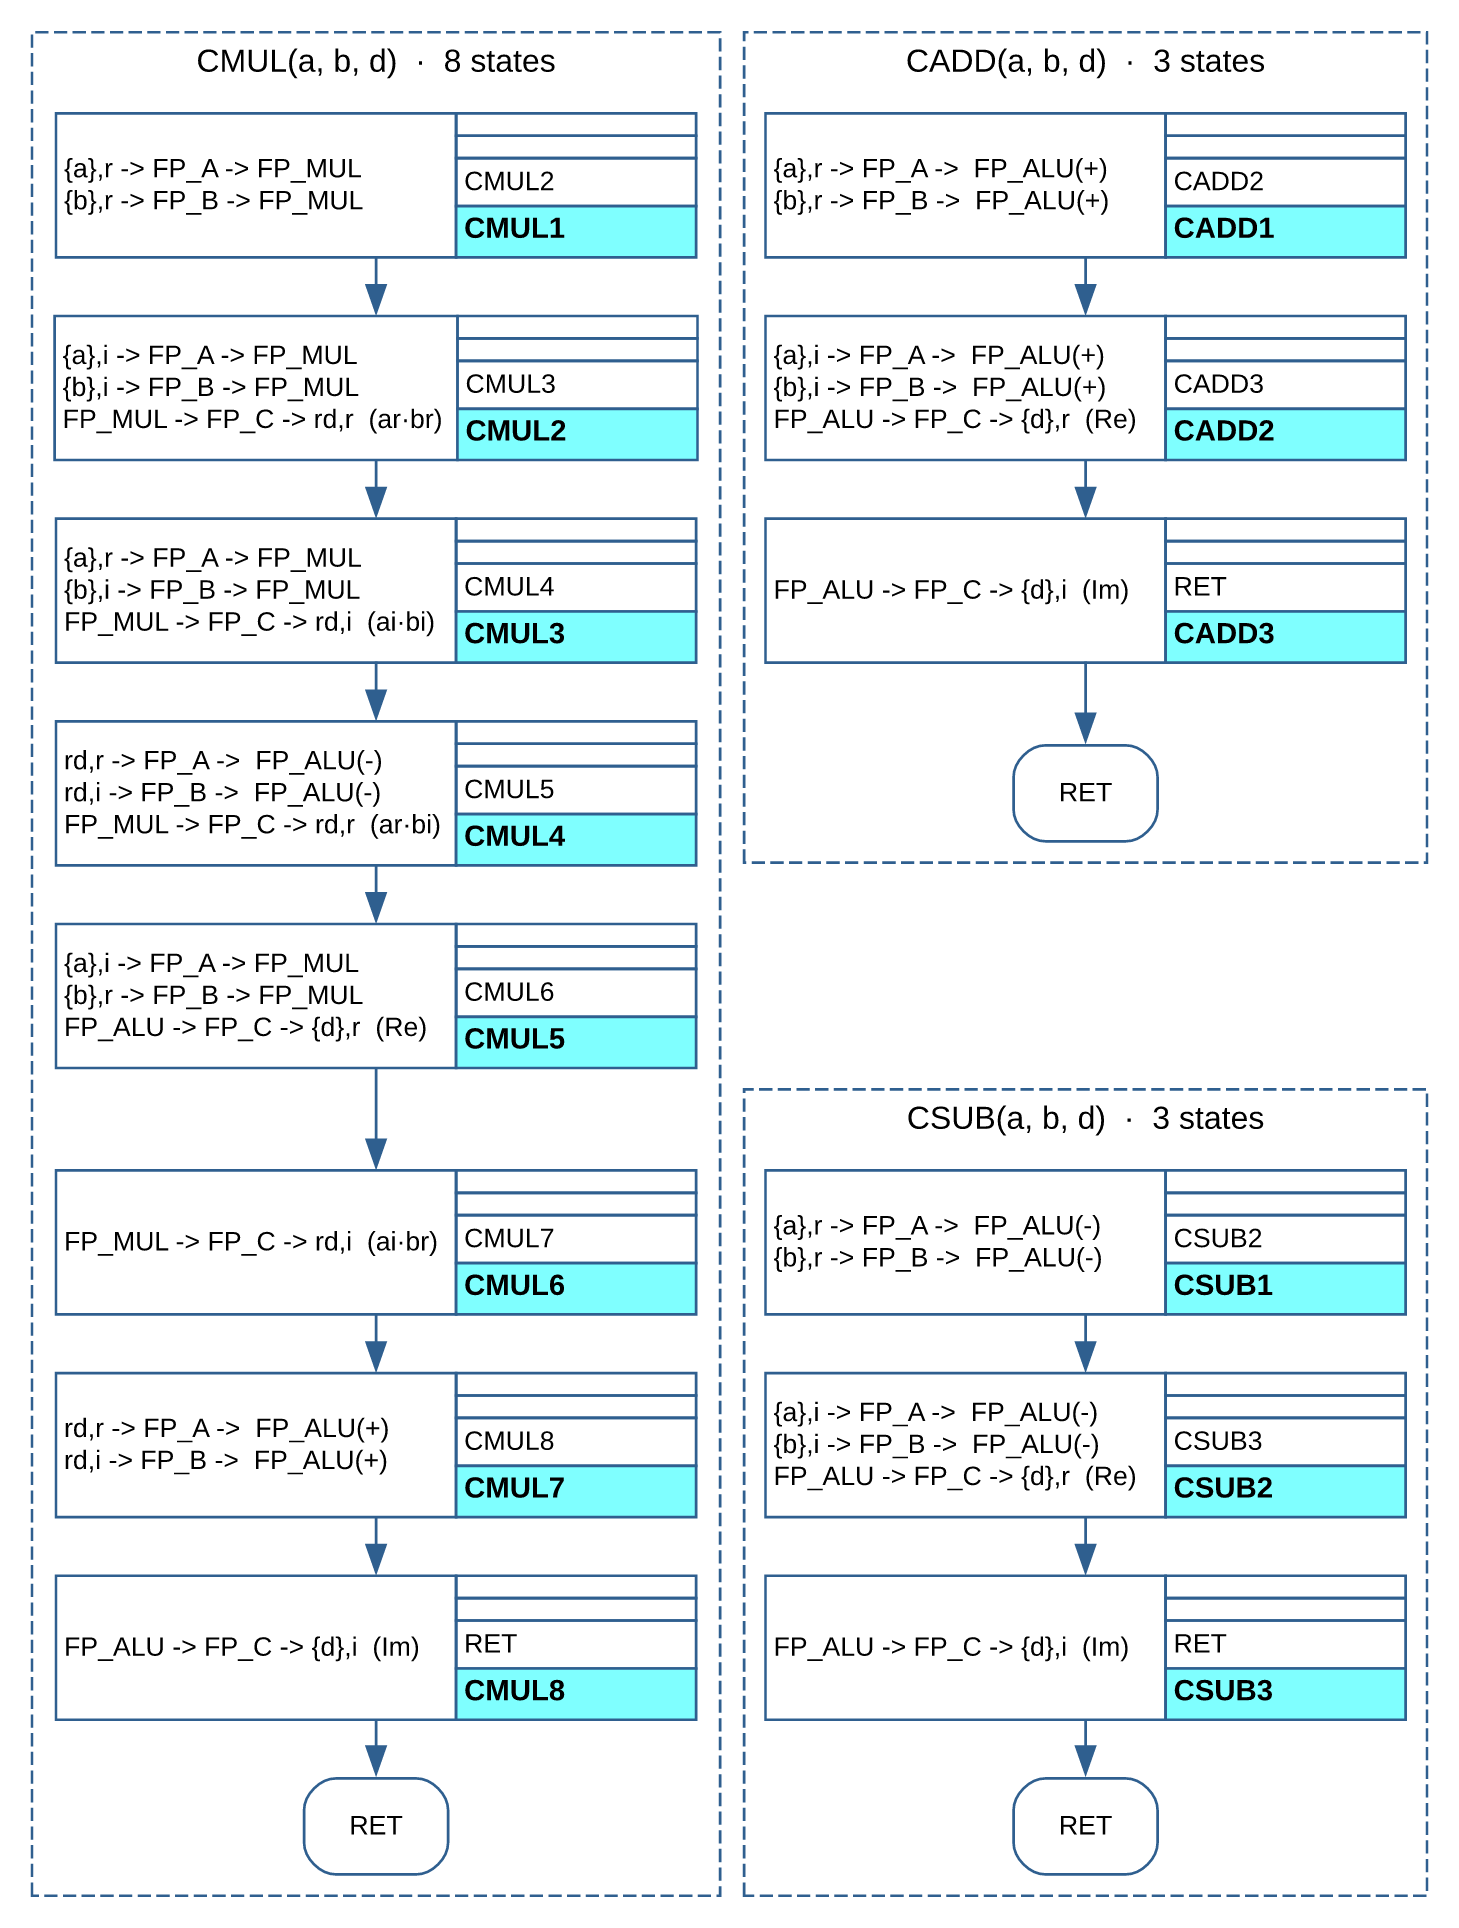
\includegraphics[width=0.8\textwidth]{pics/fsm_live/Complex_substates_FP_A_FP_B_operands_FP_C_write-back_scratch_rd_.png}
\end{figure}

In der weiteren Registertransferfolge \ref{fig:unoptimized_FSM_RFD} ist der
Zustandsautomat und die benötigten Transfere für die unoptimierte
Datenpfadarchitektur dargestellt. Die im vorherigen Kapitel definierten
Funktionen werden dabei aus Übersichtsgründen nur aufgerufen, in einer
implementierten FSM müssten sie aber direkt in die eigentliche FSM eingefügt
werden.

\begin{figure}
	\centering
	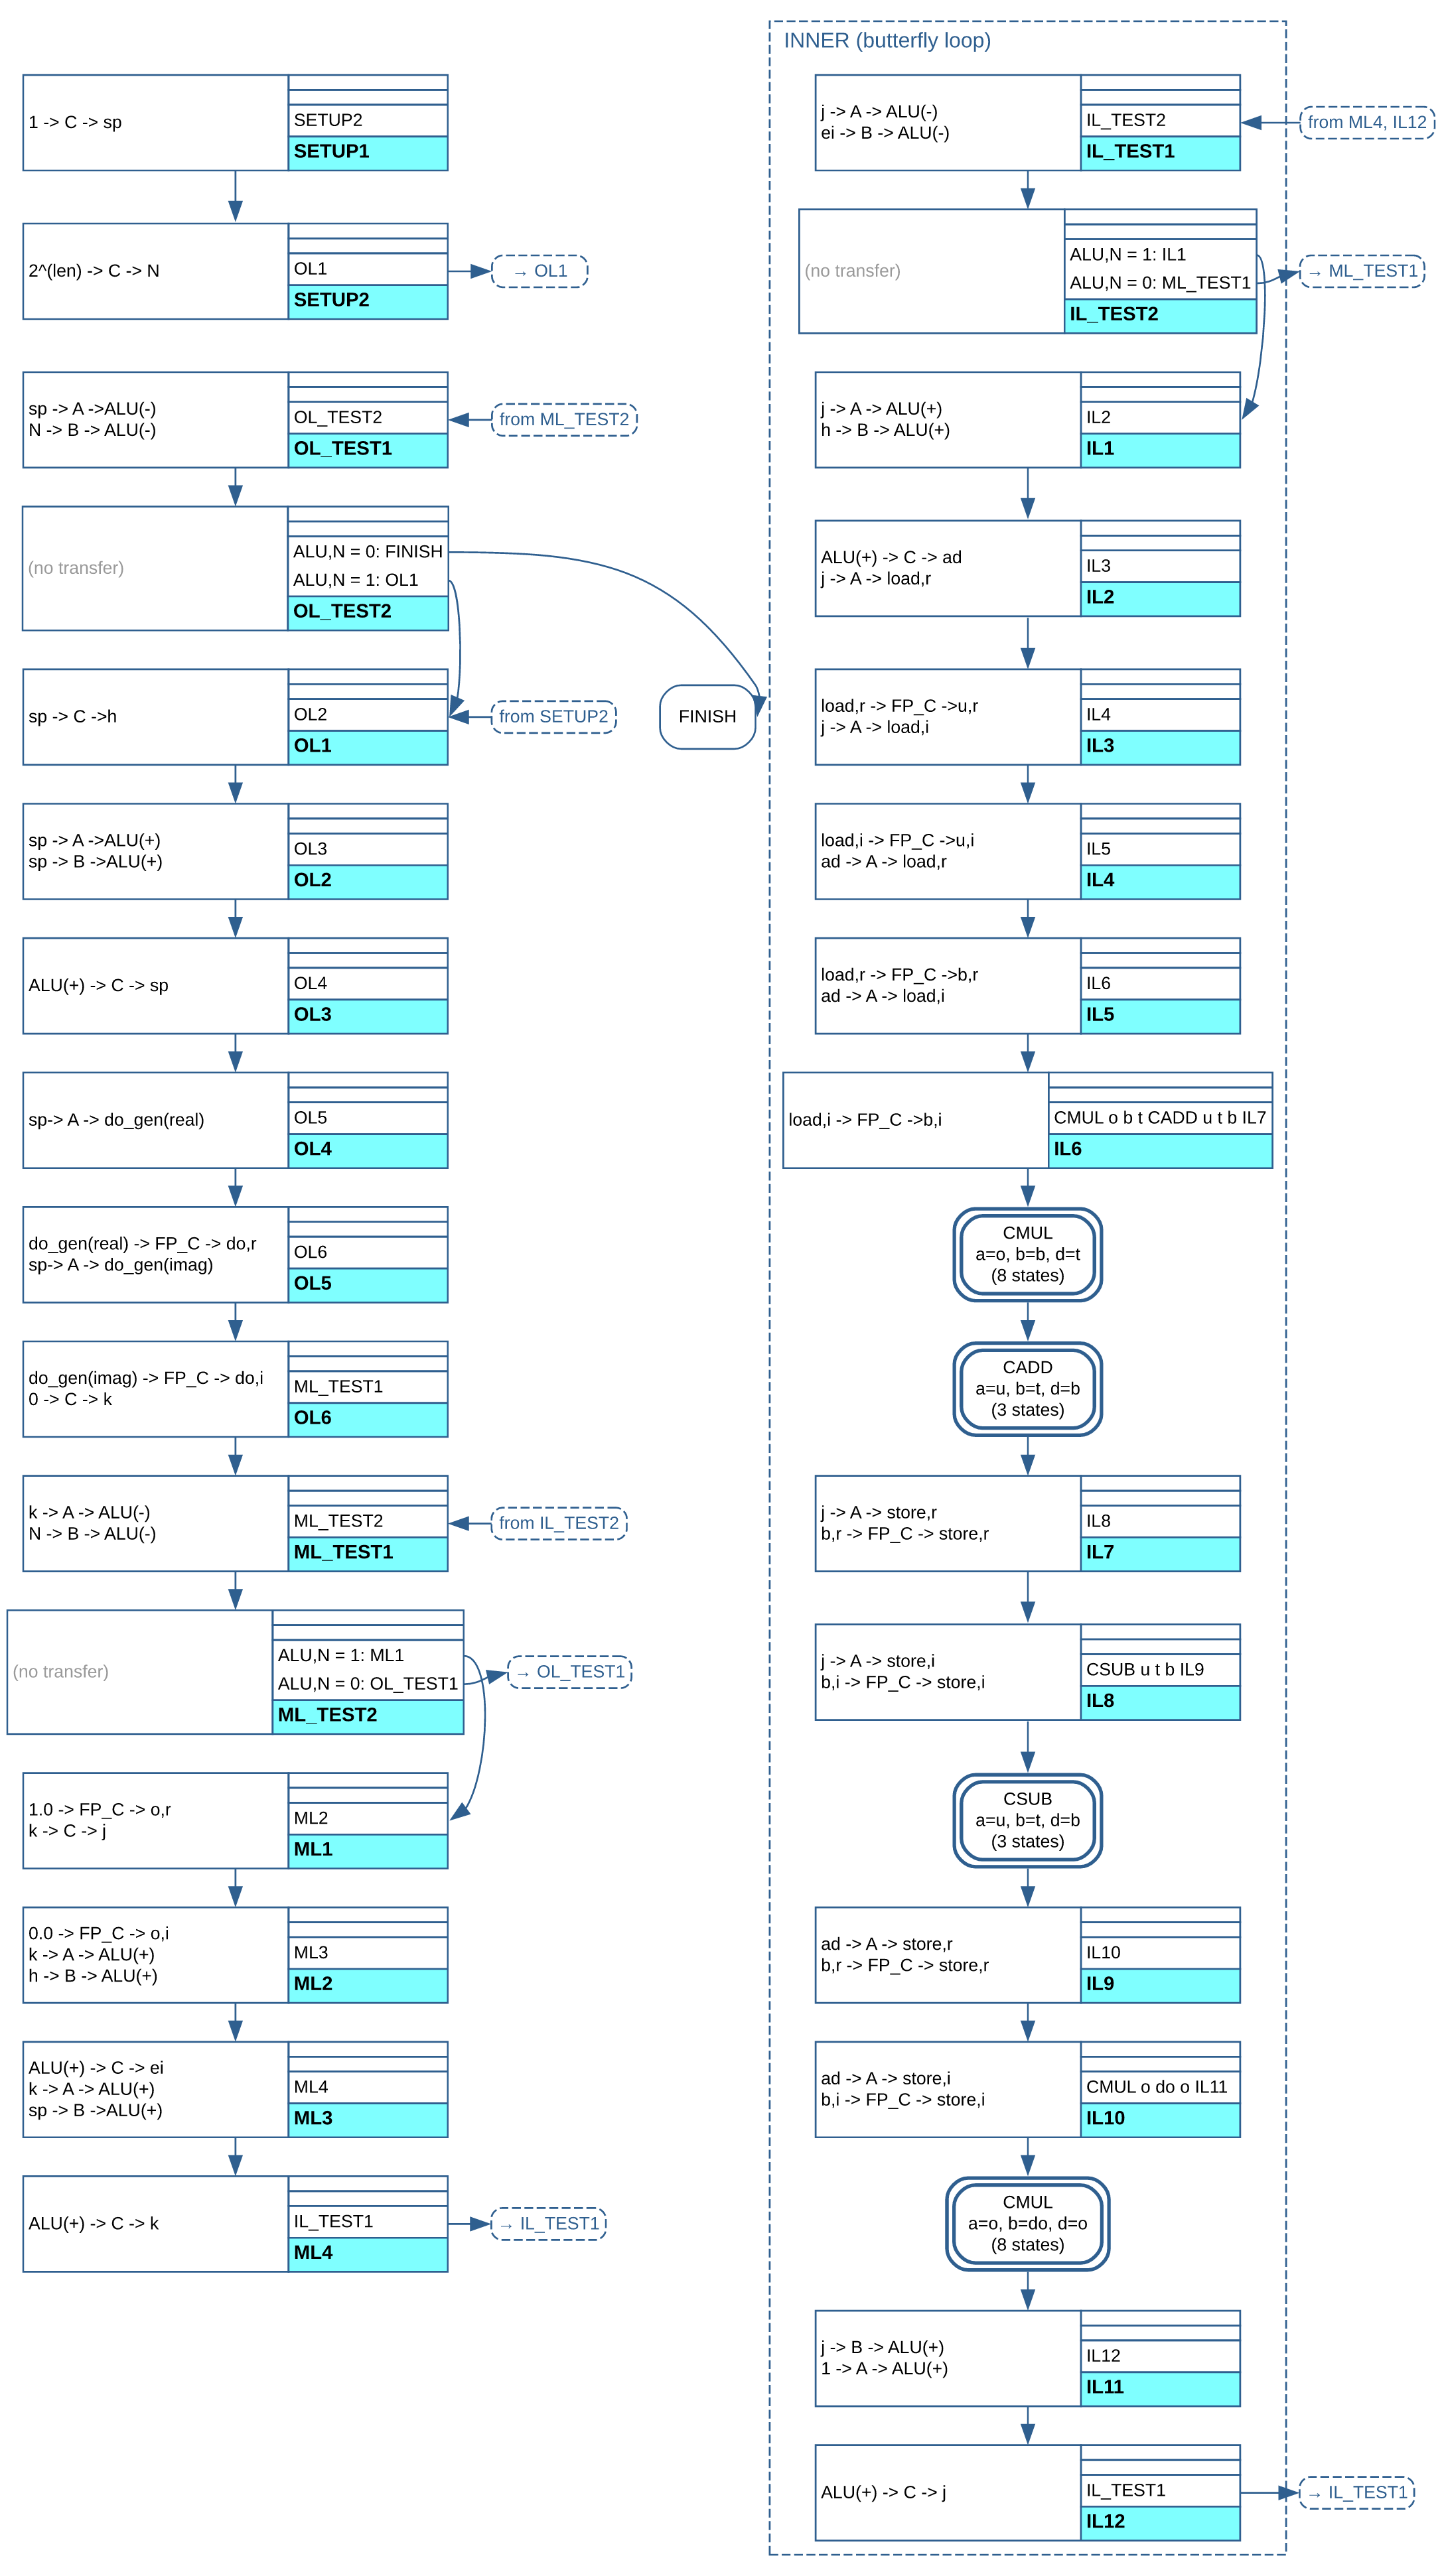
\includegraphics[width=0.8\textwidth]{pics/fsm_live/FFT.png}
	\label{fig:unoptimized_FSM_RFD}
\end{figure}

\subsection{Optimierungen}
Das primäre Optimierungskriterium in dieser Arbeit ist Geschwindigkeit, der
ASIC muss dafür also eine iteration des inneren loops so schnell wie möglich
ausführen. Durch die unoptimierte FSM ist deutlich geworden, wie viel Takte
eine einzelne Iteration der inneren Schleife dauern würde. Aus Gründen der
Übersichtlichkeit und Länge der Arbeit wird hier darauf verzichtet, eine
Registertransferanalyse vom ersten Datenpfad darzustellen anstelle dessen
führen wir zuerst Optimierungen ein. Um die Anzahl der Zustände zu verringern
und die Verarbeitungsgeschwindigkeit zu erhöhen wechseln wir auf einen
Datenpfad, der direkt mit komplexen Zahlen arbeiten kann. Dafür halten alle
Register, welche eine komplexe Zahl speichern 128 Bit, je 64 für Imaginär- und
Realteil. Daraus folgen drei Konsequenzen: Zum einen muss das Speicherinterface
128 Bit Daten lesen und schreiben können, wobei wir einen dual-port Speicher,
welcher gleichzeitig schreiben und lesen kann verwenden. Es müssen aber auch
Komplexe Addition/Subtraktion und Multiplikation mit komplexen Zahlen arbeiten
können. Um dies zu erreichen erstellen wir 2 neue Datenpfadelemente,
dargestellt in Diagramm \ref{fig:COMP_ALU_DP} und \ref{fig:COMP_MUL_DP}. Die
komplexe ALU kann wie ein normales Datenpfadelement verwendet werden und
benötigt nur einen Takt, die komplexe Multiplikation hingegen benötigt 2 Takte,
bis ein valides Ergebnis am Ausgang erscheint. Durch die Register am Ende der
internen Gleitkomma-Multiplizierer, kann man aber jeden Takt eine neue
Berechnung starten. Der erstellte komplexe Gleitkomma Multiplizierer hat einen
großen Flächenverbrauch, da er 4 Gleitkomma Multiplizierer enthält, welche
schon im unoptimierten Datenpfad die Einheiten mit dem größten Flächenverbrauch
waren. Das primäre Optimierungskriterium dieser Arbeit ist jedoch
Geschwindigkeit und wie später noch gezeigt wird, erreicht der ASIC final eine
hundertprozentige Auslastung des komplexen Multiplizierers in der mittleren und
inneren Schleife.

\begin{figure}[ht]
	\centering
	\begin{subfigure}[b]{0.3\textwidth}
		\centering
		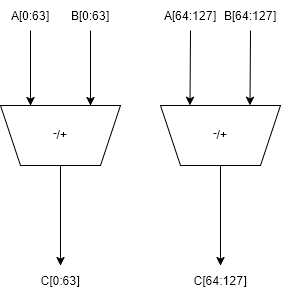
\includegraphics[width=\linewidth]{pics/Complex ALU.drawio.png}
		\caption{Komplexe ALU}
		\label{fig:COMP_ALU_DP}
	\end{subfigure}
	\hfill
	\begin{subfigure}[b]{0.6\textwidth}
		\centering
		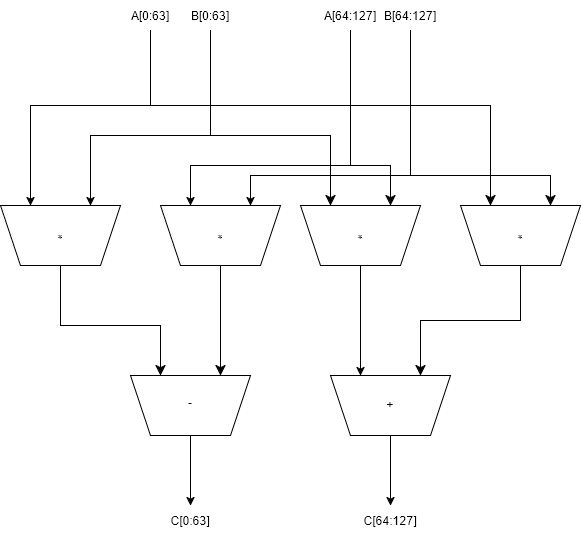
\includegraphics[width=\linewidth]{pics/Complex MUL.drawio.png}
		\caption{Komplexer Multiplizierer}
		\label{fig:COMP_MUL_DP}
	\end{subfigure}
	\caption{Komplexe Datenpfadelemente}
	\label{fig:COMP_DP}
\end{figure}

\subsection{Unoptimierter komplexer Datenflussgraph}
In Diagramm \ref{fig:complex_unoptimized_datapath} ist der modifizierte
Datenpfad dargestellt, welcher jetzt die komplexen Operationen nutzt.
\begin{figure}
	\centering
	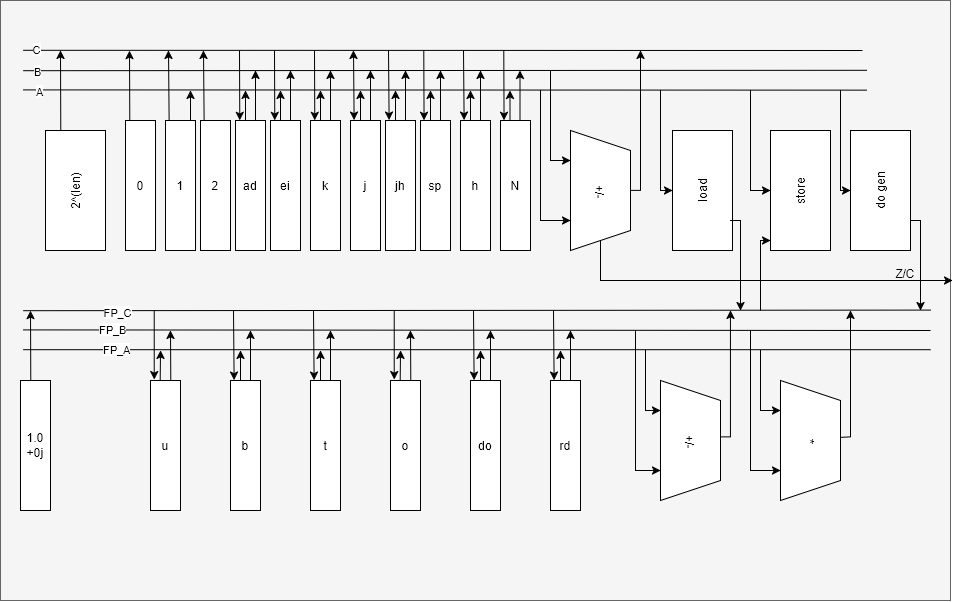
\includegraphics[width=0.8\textwidth]{pics/Complex Datapath architecture.png}
	\label{fig:complex_unoptimized_datapath}
\end{figure}
\subsection{Unoptimierte komplexe FSM}
Mithilfe des komplexen Datenpfades und einiger kleinerer optimierungen in den
Schleifen, erhält man das Registerfolgediagram
\ref{fig:unoptimized_complex_FSM_RFD}

\begin{figure}
	\centering
	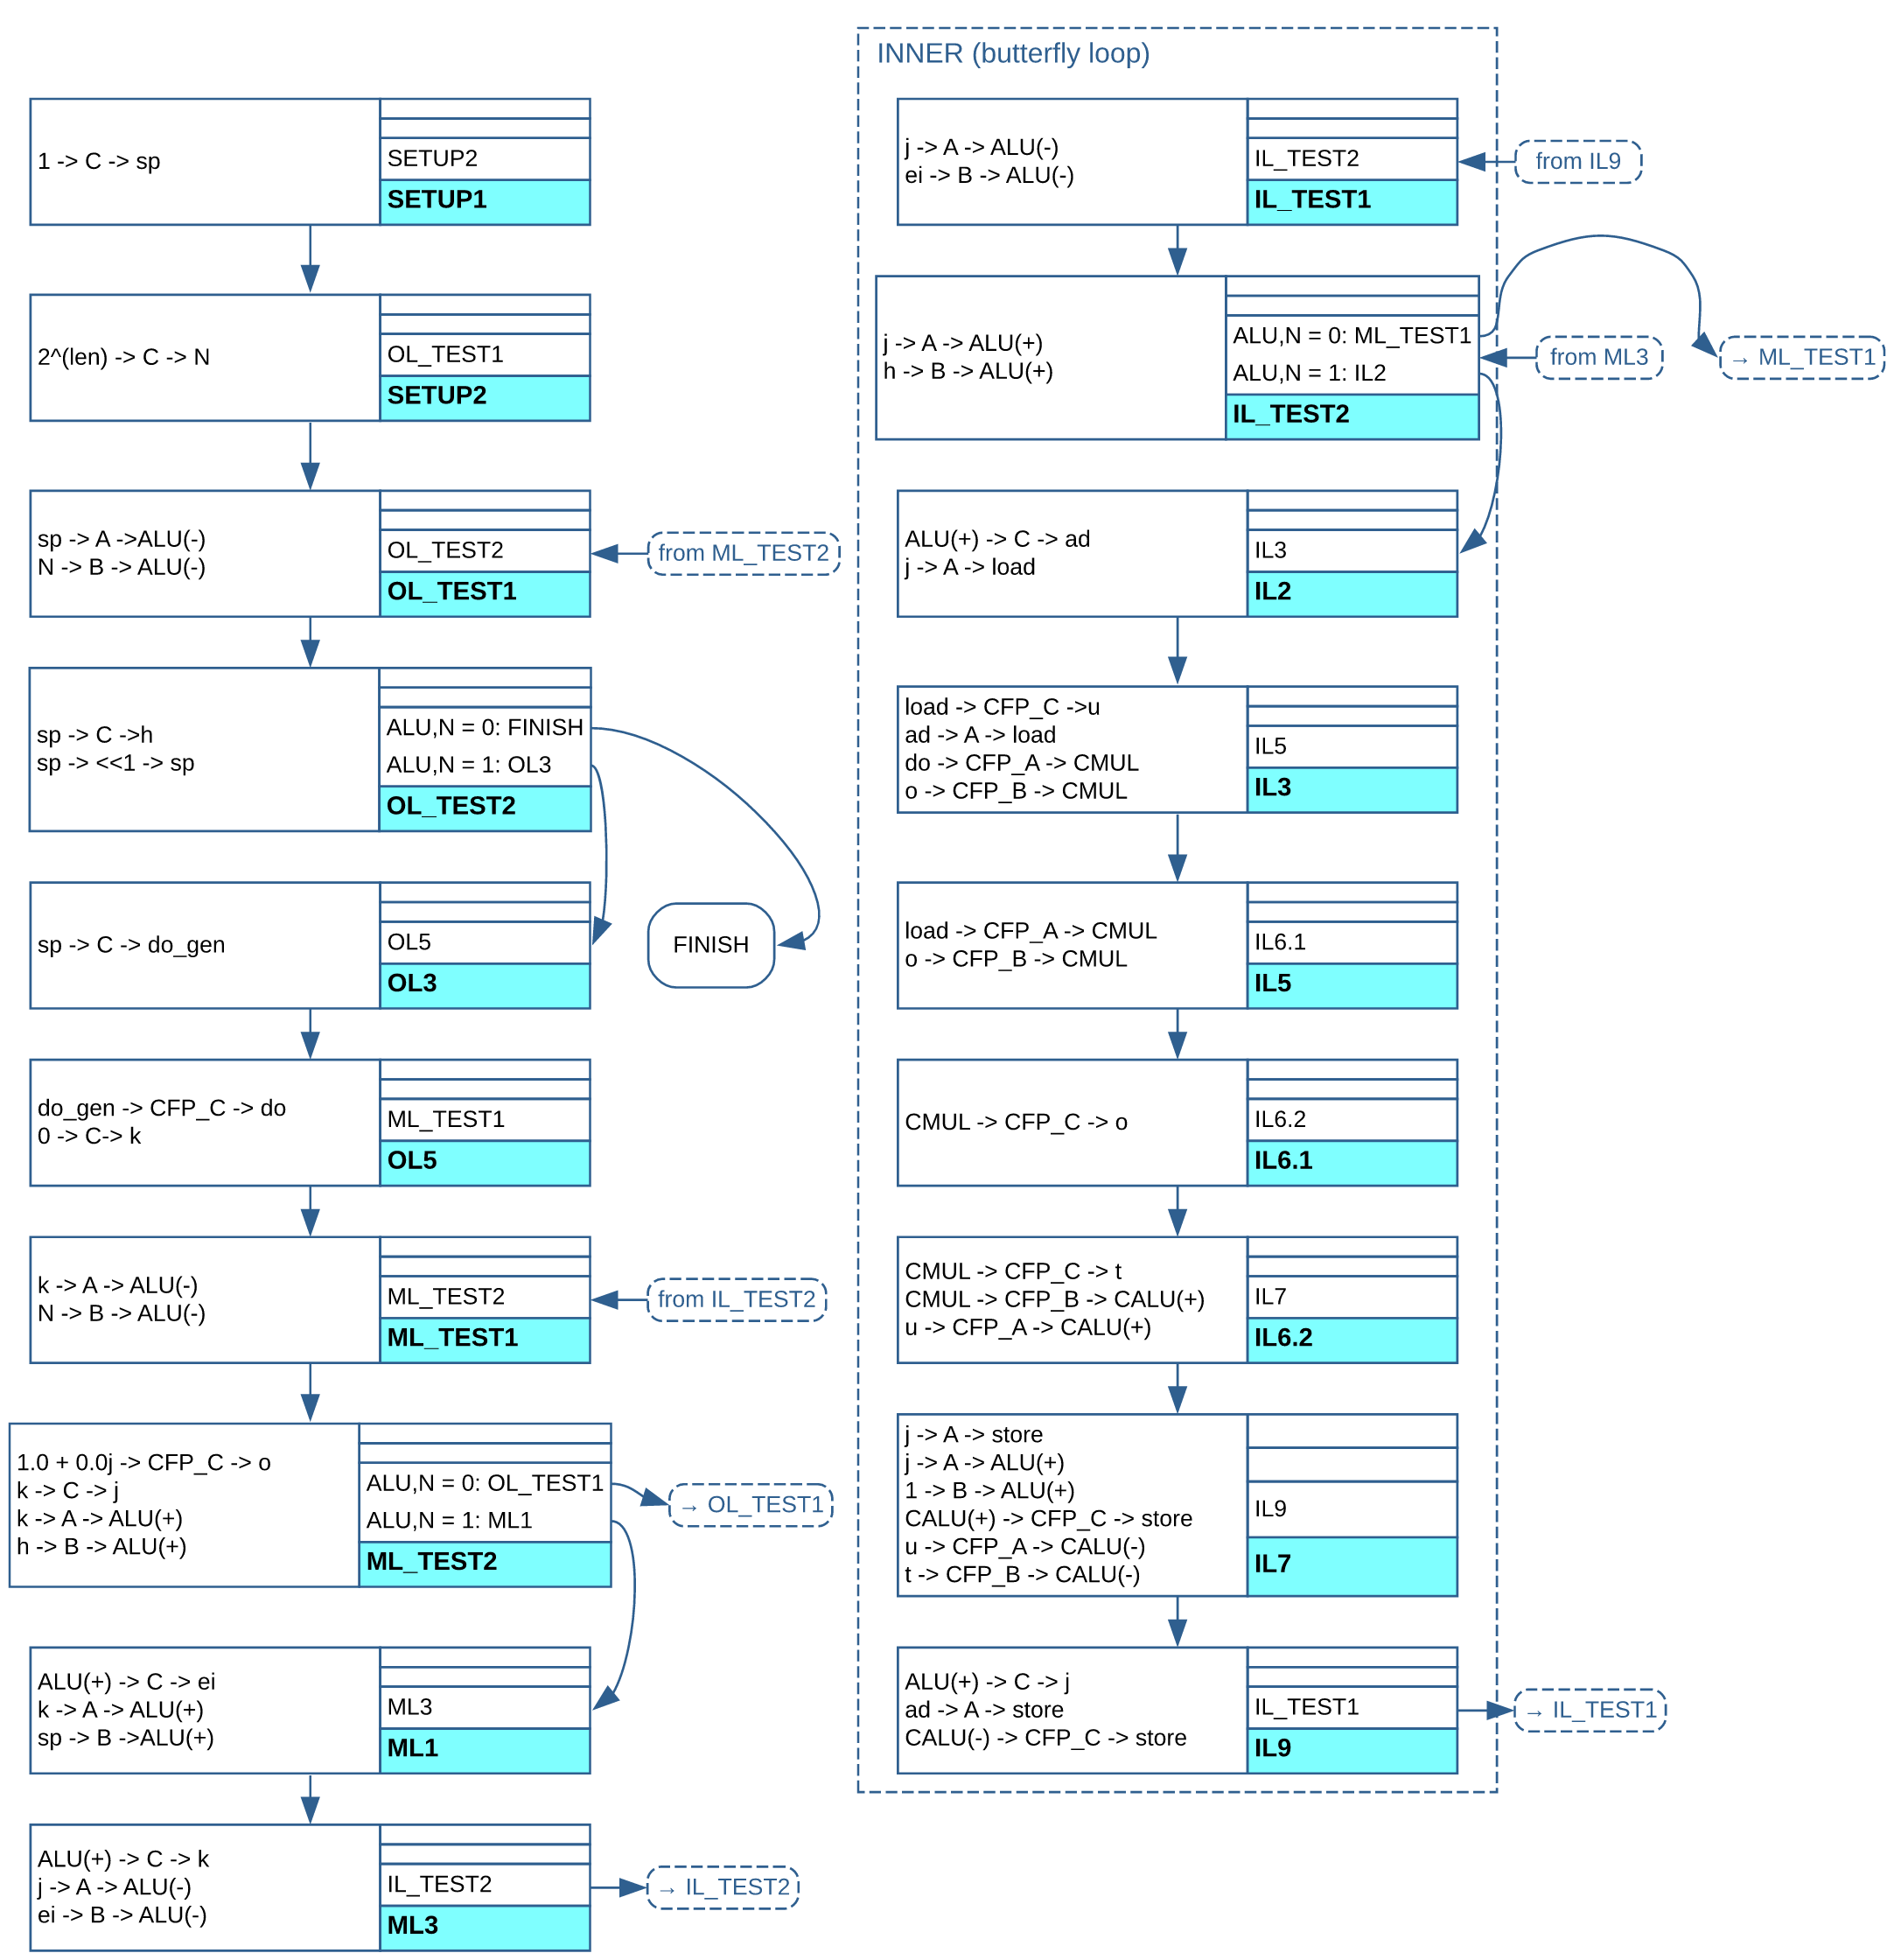
\includegraphics[width=0.8\textwidth]{pics/fsm_live/FFT_RFD_complex.png}
	\label{fig:unoptimized_complex_FSM_RFD}
\end{figure}

\subsection{Optimierter Datenflussgraph}
Auch erklären, was das Optimierungskriterium ist.

\subsection{Datenpfadarchitektur}
In \autoref{table:datentransfer} sind die Datentransferoperationen für die
Register, Recheneinheiten und den Speicher aufgelistet. Sie wurden aus dem
Datenflussgraphen abgeleitet. Zeigt mehr als eine Quelle auf ein
Datenpfadelement, wird ein Multiplexer benötigt.

\begin{table}[ht]
	\centering
	\begin{tabular}{|l|l|l|l|l|l|l|l|l|l|}\hline
		Ziel        & Quellen    & 1       & 2  & 3   & 4  & 5   & 6    & 7  & 8  \\ \hline \hline
		R1          & \leftarrow & 0       & T1 &     &    &     &      &    &    \\ \hline
		R3          & \leftarrow & 0       & T1 &     &    &     &      &    &    \\ \hline
		RR          & \leftarrow & 0       & T1 &     &    &     &      &    &    \\ \hline
		RC          & \leftarrow & 0       & T1 &     &    &     &      &    &    \\ \hline
		R2          & \leftarrow & 0       & T2 &     &    &     &      &    &    \\ \hline
		R4          & \leftarrow & 0       & T2 &     &    &     &      &    &    \\ \hline
		RCX         & \leftarrow & T1      &    &     &    &     &      &    &    \\ \hline
		RCY         & \leftarrow & T1      &    &     &    &     &      &    &    \\ \hline
		RD          & \leftarrow & T3      &    &     &    &     &      &    &    \\ \hline
		Rres        & \leftarrow & MEM(DO) &    &     &    &     &      &    &    \\ \hline
		Riter       & \leftarrow & MEM(DO) &    &     &    &     &      &    &    \\ \hline
		RI          & \leftarrow & Riter   & T4 &     &    &     &      &    &    \\ \hline
		Radr        & \leftarrow & T4      &    &     &    &     &      &    &    \\ \hline
		MEM(ADR)    & \leftarrow & Radr    &    &     &    &     &      &    &    \\ \hline
		MEM(DI)     & \leftarrow & RI      &    &     &    &     &      &    &    \\ \hline
		ALU(1)      & \leftarrow & T1      & T2 & 2   & RC & R2  & Rres & RR &    \\ \hline
		ALU(2)      & \leftarrow & T2      & 2  & RCY & R4 & RCX & 1    & 4  & T1 \\ \hline
		MUL(1)      & \leftarrow & 2       & RD & T1  & T2 &     &      &    &    \\ \hline
		MUL(2)      & \leftarrow & RR      & RC & R3  & R1 & T1  &      &    &    \\ \hline
		DIV(1)      & \leftarrow & 4       &    &     &    &     &      &    &    \\ \hline
		DIV(2)      & \leftarrow & MEM(DO) &    &     &    &     &      &    &    \\ \hline
		ALU\_INT(1) & \leftarrow & Radr    & RI &     &    &     &      &    &    \\ \hline
		ALU\_INT(2) & \leftarrow & CInt 1  &    &     &    &     &      &    &    \\ \hline
	\end{tabular}
	\caption{Datentransferoperationen der Datenpfadarchitektur. Bei Konstanten wurde auf das Präfix \textit{Const} verzichtet.}
	\label{table:datentransfer}
\end{table}

Anschließend wurde die Datenpfadarchitektur erstellt. Als Bild genügt hier der
Ausdruck aus Cadence.

\subsection{Registertransferfolgen}
In \autoref{fig:register} seht ihr ein Beispiel der Registertransferfolgen, als
formschöne Vektorgrafik. Erstellt in drawio. Für den Export wurden die
Einstellungen in \autoref{fig:screenshot} verwendet.

\begin{figure}[ht]
	\centering
	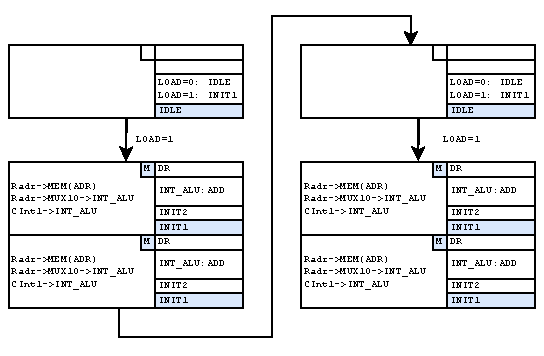
\includegraphics[width=\textwidth]{pics/Registertransferfolge-optimized.drawio.pdf}
	\caption{Registertransferfolgen. Erstellt mit drawio. Source befindet sich in dieser zip Datei.}
	\label{fig:register}
\end{figure}

\begin{figure}[ht]
	\centering
	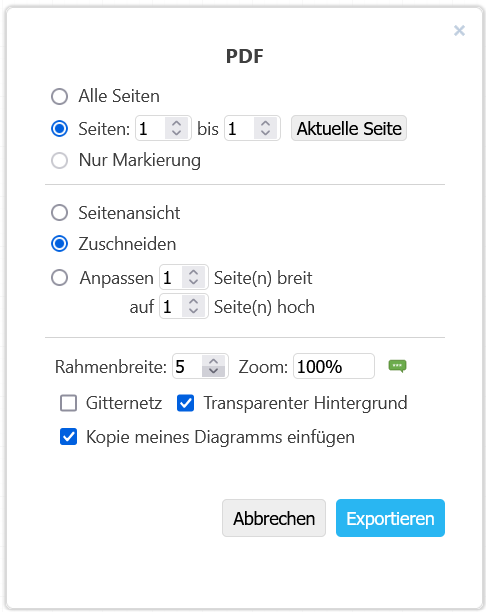
\includegraphics[width=0.6\textwidth]{pics/Screenshot 2025-01-12 190121.png}
	\caption{Exporteinstellungen drawio.}
	\label{fig:screenshot}
\end{figure}
\clearpage

\subsection{Zustandsgraph}
Nicht vergessen: Die Zustandskodierung, wie in \autoref{table:zustandskot}
dargestellt.

\begin{table}[ht]
	\centering
	\begin{tabular}[t]{|l|l|}
		\hline
		Zustand & Hex-Code \\ \hline \hline
		IDLE    & 00       \\ \hline
		INIT1   & 01       \\ \hline
		INIT2   & 02       \\ \hline
		INIT3   & 03       \\ \hline
		INIT4   & 04       \\ \hline
		INIT5   & 05       \\ \hline
		INIT6   & 06       \\ \hline
		INIT7   & 07       \\ \hline
		INIT8   & 08       \\ \hline
		INIT9   & 09       \\ \hline
		RLOOP1  & 0A       \\ \hline
		RLOOP2  & 0B       \\ \hline
		RLOOP3  & 0C       \\ \hline
		CLOOP1  & 0D       \\ \hline
	\end{tabular}
	\begin{tabular}[t]{|l|l|}
		\hline
		Zustand & Hex-Code \\ \hline \hline
		CLOOP2  & 0E       \\ \hline
		CLOOP3  & 0F       \\ \hline
		ILOOP1  & 10       \\ \hline
		ILOOP2  & 11       \\ \hline
		ILOOP3  & 12       \\ \hline
		ILOOP4  & 13       \\ \hline
		ILOOP5  & 14       \\ \hline
		ILOOP6  & 15       \\ \hline
		ILOOP7  & 16       \\ \hline
		CLOOP4  & 17       \\ \hline
		CLOOP5  & 18       \\ \hline
		CLOOP6  & 19       \\ \hline
		RLOOP4  & 1A       \\ \hline
		RLOOP5  & 1B       \\ \hline
		RLOOP6  & 1C       \\ \hline
	\end{tabular}
	\caption{Zustandskodierung}
	\label{table:zustandskot}
\end{table}

\subsection{Gesamtschaltung}

\section{Simulation}
In den folgenden Unterkapiteln wurde die Gesamtschaltung mithilfe der Verilog
Testbench simuliert. Dafür müssen die beiden Simulationsparameter
\textit{resolution} und \textit{iteration count} im Speicher liegen. Diese
werden in eine Textdatei geschrieben, welche anschließend von der Testbench
eingelesen werden. Es wurden folgende Simulationsparameter verwendet:

\begin{table}[ht]
	\centering
	\begin{tabular}{|l|l|l|l|}
		\hline
		Parameter                & Dezimal & Hexadezimal & Adresse im Speicher \\ \hline\hline
		\textit{resolution}      & 25      & 0x00000019  & 0x00000000          \\ \hline
		\textit{iteration count} & 50      & 0x00000032  & 0x00000001          \\ \hline
	\end{tabular}
\end{table}

\subsection{Verifikation}
Wie habt ihr Sichergestellt, dass euer Algorithmus tut, was er tut?

\subsection{Schaltungssynthese}

\subsection{Layoutsynthese}

\section{Zusammenfassung}
Die Simulation des Schaltkreises hat gezeigt, dass er wie erwartet
funktioniert. Ihr solltet noch ein paar Worte sagen zu:
\begin{itemize}
	\item Abweichungen zur Referenzimplementierung
	\item Trade-off Geschwindigkeit - Area
	\item Verbesserungsmöglichkeiten
\end{itemize}
Eine halbe Seite genügt.

\clearpage
\begin{appendices}
	\begingroup
	\let\clearpage\relax% Remove \clearpage functionality
	\section{Quellcode}
	\subsection{Referenzimplementierung}\label{appendix:Referenzimplementierung}
	\lstinputlisting[style=CodeStyle,language=C]{code/helloworld.c}
	\subsection{FSM}\label{appendix:fsm}
	%\lstinputlisting[style=CodeStyle,language=Verilog]{code/FSM.v}
	\subsection{Controllogic}\label{appendix:controllogic}
	%\lstinputlisting[style=CodeStyle,language=Verilog]{code/Controllogic.v}
	\endgroup %The definition of \clearpage is restored after \endgroup as it adheres to the scoping rules of a redefinition within a group.

	\clearpage

	\begingroup
	\let\clearpage\relax% Remove \clearpage functionality
	\section{Reports}\label{appendix:reports}
	\subsection{Area}
	%\lstinputlisting[language={},basicstyle=\footnotesize,breaklines=true]{reports/fc_example.report_area}
	\subsection{Power}
	%\lstinputlisting[language={},basicstyle=\footnotesize,breaklines=true]{reports/fc_example.report_power}
	\subsection{Timing}
	%\lstinputlisting[language={},basicstyle=\footnotesize,breaklines=true]{reports/fc_example.report_timing}
	\endgroup %The definition of \clearpage is restored after \endgroup as it adheres to the scoping rules of a redefinition within a group.
\end{appendices}

\clearpage
\printbibliography
\end{document}
